% !TeX encoding = UTF-8
% !TeX root = ./main.tex

\reviewer{}

\begin{question}
\lipsum[1][1-5]
\end{question}

\response
\lipsum[1][6]

\begin{question}
\lipsum[2][1-5]
\end{question}

\response
\lipsum[2][6-10]
\lipsum[2][11], as shown in Fig.~\ref{fig_1}.
\begin{figure}[ht]
    \centering 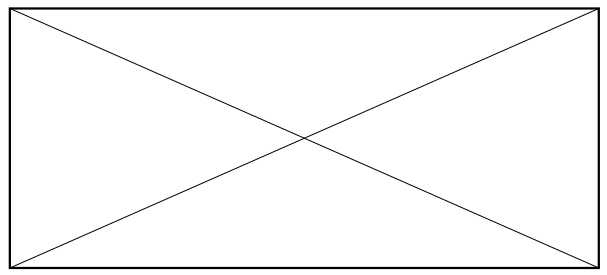
\includegraphics[scale=0.5]{figure_1}
    \caption{\lipsum[2][12]}
%    \vspace{-2ex}
    \label{fig_1}
\end{figure} 

\lipsum[3][1]~\cite{doe2021Title1}.
\lipsum[3][2]~\cite{doe2021Title2,bourne2021Title3}.
\lipsum[3][3] in Table~\ref{table_1}. 

\begin{table}[!h]
	% increase table row spacing, adjust to taste
	% \renewcommand{\arraystretch}{1.3}
	% if using array.sty, it might be a good idea to tweak the value of
	% \extrarowheight as needed to properly center the text within the cells
	\caption{Table Caption}
%    \vspace{-2ex}
	\label{table_1}
	\centering
	% Some packages, such as MDW tools, offer better commands for making tables
	% than the plain LaTeX2e tabular which is used here.
	\begin{tabular}{c c c c}
		\hline\hline \\ [-3mm]
		Item1    & Item2     & Item3   & Item4 \\ 
		\hline
		A & B & C & D \\
		E & F & G & H \\
		\hline\hline \\ [-3mm]
    \end{tabular}
\end{table}

\lipsum[3][4-8]
The amendment is as follows:
\begin{amendment}{SectionNum}{Title of the Section}
\lipsum[4][1-10]

\begin{figure}[H]
    \centering
    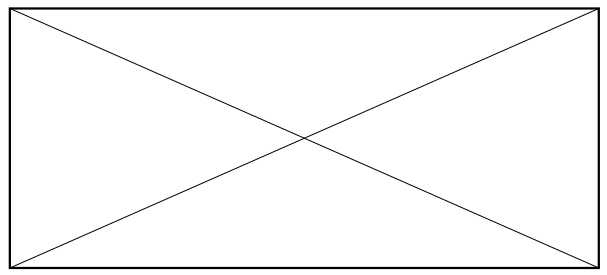
\includegraphics[scale=0.5]{figure_2}
	\caption*{Fig. X: The numbering of all figures and tables in the \textit{amendment} environment must be mannual.}
    \label{fig_ame_1}
\end{figure}
\end{amendment}


\bibliographystyle{IEEEtran}
\bibliography{ref}
